\section{{\tool}: Approach Overview}
\label{overview:sec}

%{\tool} has two main processes: training and predicting.


\subsection{Training Process}

Figure~\ref{overview-training} shows the overview of our training
process. We use a divide-and-conquer strategy for each buggy method:
if a method has multiple buggy statements, we process one buggy
statement at a time and its enclosing method, together with its
respective fixed code as a training instance.
%The input of~this process is the source code of a buggy method and one
%of its buggy statements, and the respective fixed source code.
The output includes the trained CCL and trained CTL models.
The training process has two main steps:

\begin{figure}[t]
	\centering
	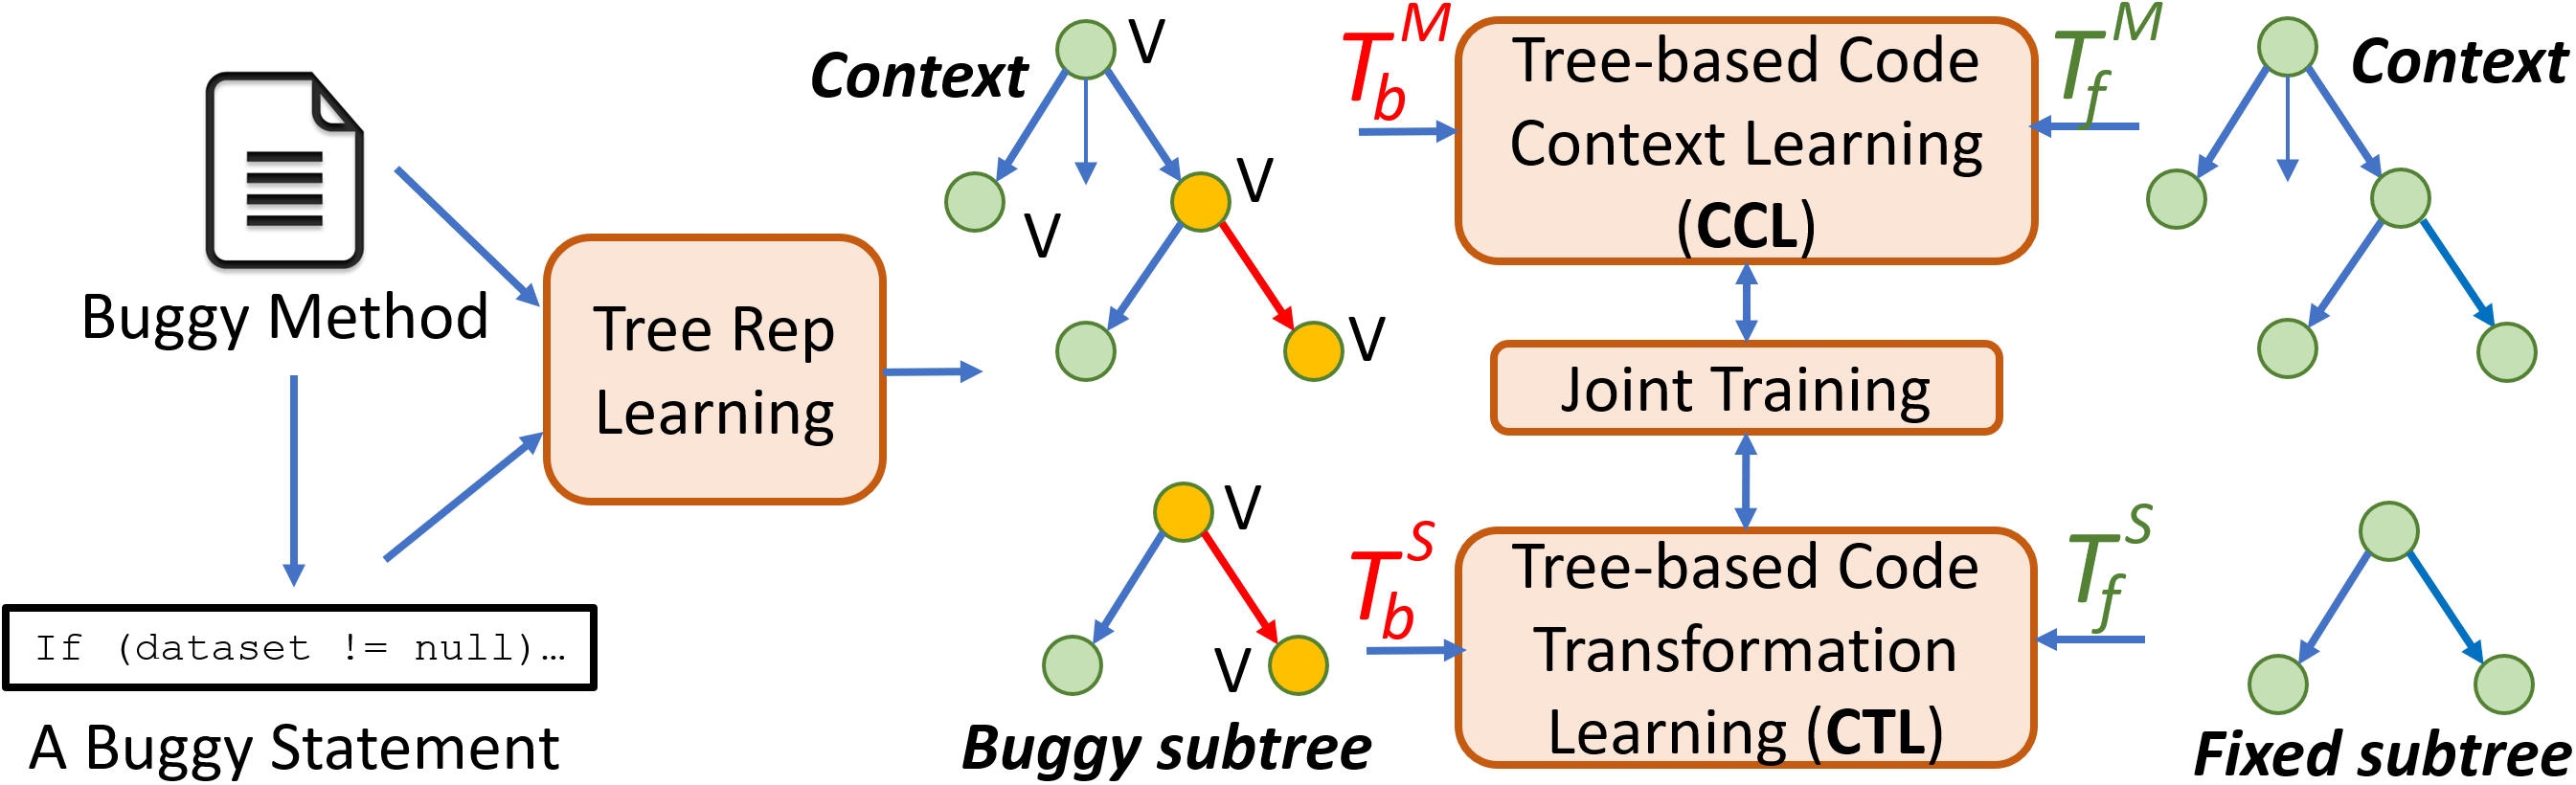
\includegraphics[width=3.4in]{graphs/new_overview-4.png}
%        \vspace{-9pt}
	\caption{{\tool}: Training Process}
	\label{overview-training}
%	\vspace{-10pt}
\end{figure}

%\vspace{2pt}
%\noindent {\bf Tree-based Representation Learning.}

\subsubsection{Tree-based Representation Learning}

{\tool} takes the source code and builds the vectors to be the inputs
of CCL and CTL. To achieve that, the given method is parsed to obtain
its AST and the subtree for the buggy statement.  Then, a word
embedding technique is used to produce the vector for each node in the
AST when we flatten the AST into a sequence. After this, we obtain the
AST for the method and the AST subtree for the buggy statement in
which {\em each node is replaced by its embedding vector}.

To build the context, we leverage the known buggy statement $s$ by
collecting the AST nodes having {\em data and control dependencies
  with $s$}. Our rationale is that the nodes having such dependencies
with $s$ provide the context for the bug fix.
%
We then take the subtree that covers all those nodes and use it as the
context (Figure~\ref{overview-training}). This subtree $T_b^{M}$ is
used as the input for CCL in the later step.
%Code Context Learning model (CCL) in the
%later step.

For code-transformation learning, we use the AST subtree $T_b^{S}$ for
the buggy statement with the embedding vectors as the input for
Code Transformation Learning model (CTL) next.

%\vspace{2pt}
%\noindent {\bf Context-aware, Dual-Task Learning Automated Program Repair.}

\subsubsection{Context-aware, Dual-Task Learning Automated Program
  Repair}

The goal of this step is to train both the tree-based CCL and the
tree-based CTL in a joint-training manner. For CCL, the context AST
(with the embeddings) before the fix is used in the input layer and
the corresponding context AST after the fix is used in the output
layer of the CCL model. For CTL, the buggy subtree with the embeddings
is used in the input layer and the corresponding fixed subtree is used
in the output layer of the CTL model.
%The entire AST $T^{M}_b$ of the buggy method after vectorization
%(i.e., each node is a vector) is used at the input layer of CCL for
%training. The AST of the corresponding fixed method $T^{M}_f$ after
%vectorization is used at the output layer of CCL. Similarly, the AST
%subtree $T^{S}_b$ of the buggy statement after vectorization is used
%at the input layer of CTL, and the subtree $T^{S}_f$ of the
%corresponding fixed statement after vectorization is used at the
%output layer of CTL.

The CCL and CTL models are realized via attention-based \code{seq2seq}
models. We use the {\em cross-stitch unit}~\cite{misra2016cross} to
train CCL and CTL simultaneously (Section~\ref{sec: dual-learning}).
%with soft-sharing the parameters to exploit this duality.
Joint training learns the shared representations between
CCL and CTL in terms of a linear combination of the input features in
both~models.
%The output includes the trained CCL and CTL models.

\subsection{Prediction Process}

\begin{figure}[t]
	\centering
	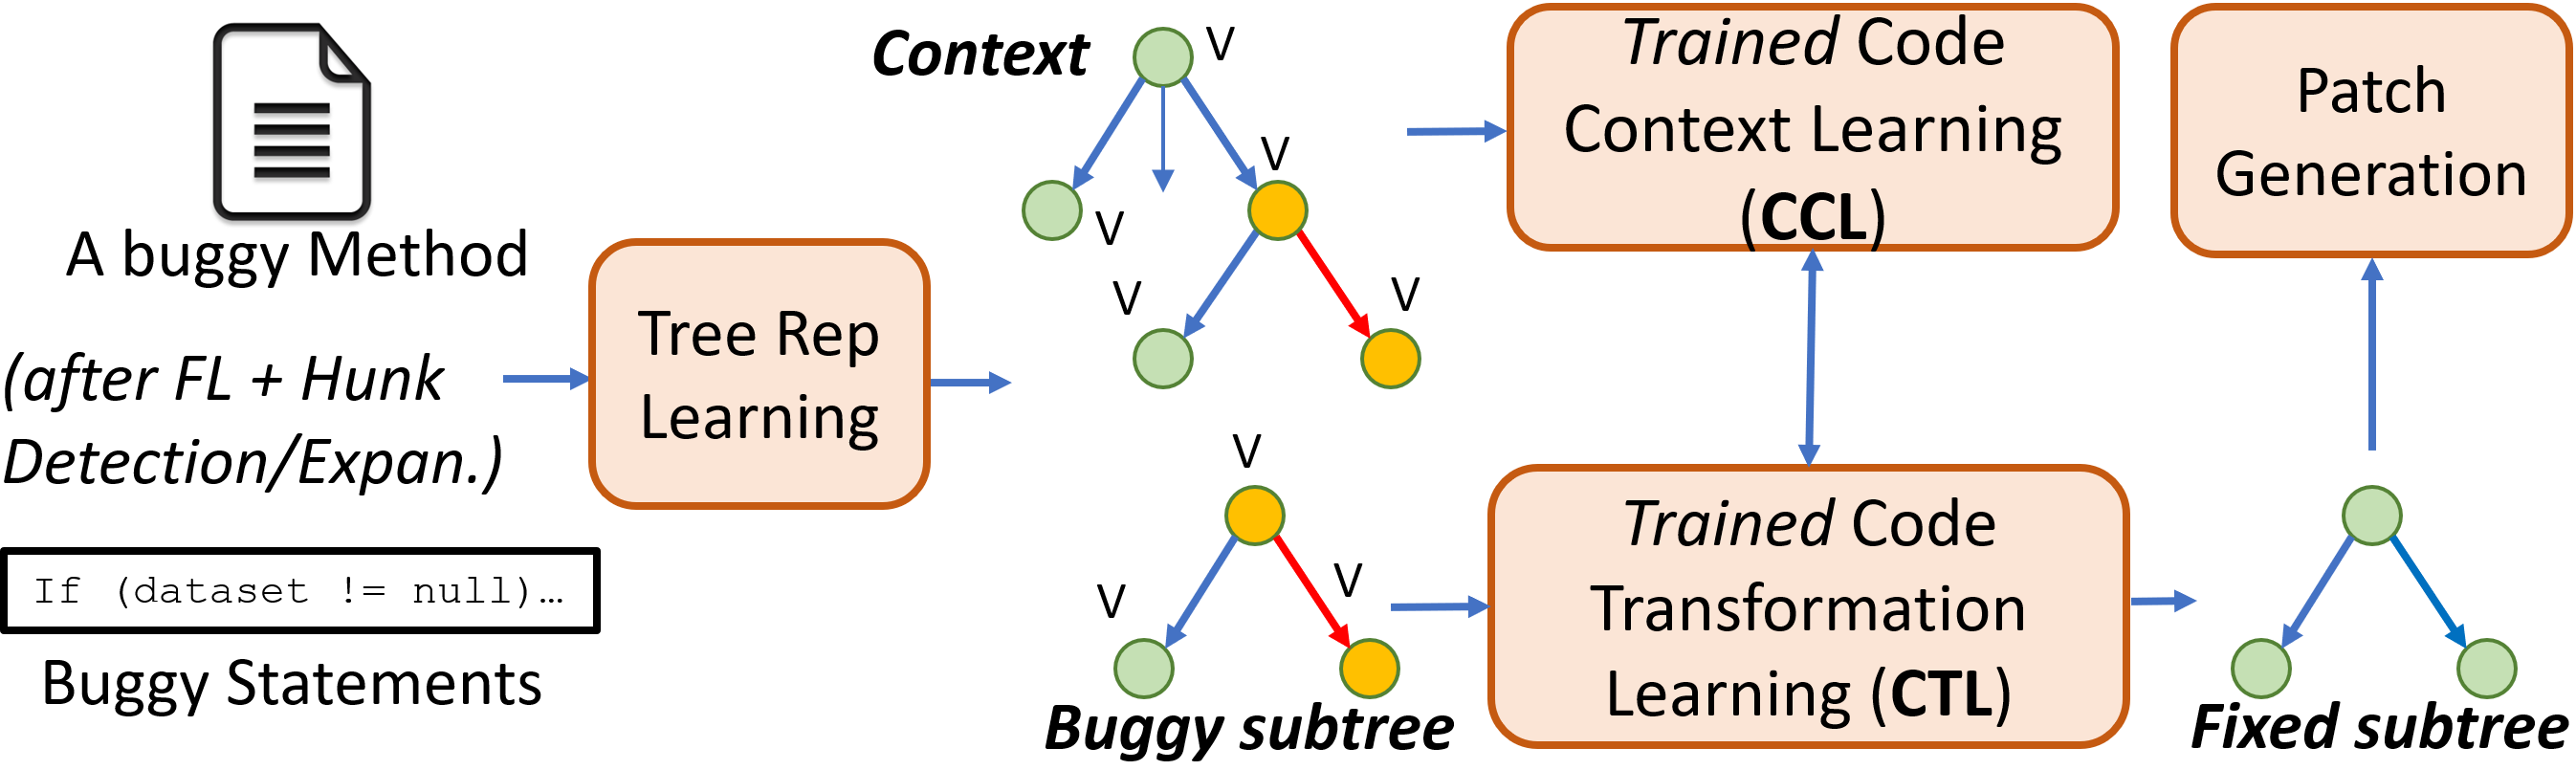
\includegraphics[width=3.3in]{graphs/overview-predict-5.png}
        \vspace{-6pt}
	\caption{{\tool}: Fixing Process}
	\label{overview-fixing}
\end{figure}

Figure~\ref{overview-fixing} illustrates the fixing process
(prediction). A fault localization (FL) tool could be used to locate
the buggy statements. We additionally use the hunk detection/expansion
module similar to DEAR~\cite{icse22} to locate
multi-hunks/multi-statements for a bug.

The hunk detection is as follows. We need to
{\em detect buggy hunk(s) that are fixed together in the same
  patch}. To do that, we fine-tune Google's pre-trained BERT
model~\cite{devlin2018bert} to learn the {\em fixing-together
  relationships among statements} using BERT's sentence-pair
classification task.
%Then, we use the fine-tuned BERT model in an algorithm to detect
%fixing-together hunks.
For training, let $H$ be a set of the hunks that are fixed together
for a bug.
%The input is all the sets $H$s for all the bugs in the
%training set.
For a pair of hunks $H_i$ and $H_j$ in $H$, we take every pair of
statements $S_k$ and $S_l$, one from each hunk, and build the vectors
for them. We consider ($S_k$, $S_l$) as ``fixed-together''. We repeat
that previous step for all such the pairs ($S_k$, $S_l$)s in $H$ and
for all $H$s, and use them to train/fine-tune the BERT model to learn
fixing-together relations among two statements in two hunks.

The fine-tuned BERT model is used for hunk detection as follows.
Ochiai~\cite{abreu2006evaluation} is run on a program $P$ to obtain
the list of buggy statements. We group the consecutive statements
within a method returned by Ochiai to form the hunks $H_1$, $H_2$,
..., $H_m$. To decide if a pair of hunks ($H_i$,$H_j$) needs to be
fixed together, for every pair of statements ($S_k$,$S_l$), one from
each hunk ($H_i$,$H_j$), we use the fine-tuned BERT model to measure
the fixing-together relationship score for ($S_k$,$S_l$). If the
average score for all the statement pairs is higher than a threshold,
we consider ($H_i$,$H_j$) as needed to be fixed together. From pairs
of hunks, we build the groups of fixing-together hunks.

Each detected hunk will be the input and fed to Tree
Representation Learning.
%A common usage of our tool is that a developer could first use a fault
%localization tool (FL) to detect the buggy statements that need to be
%fixed. Then, the input for {\tool} is a buggy statement in the
%enclosing method.
%
%The fixing process shares the Tree-based Representation
%Learning step with the training.
After this, the vectorized buggy AST subtree (a node is replaced by a
vector), is used as the input of the trained CTL model. That buggy
subtree might have smaller buggy subtrees for buggy statements.  The
output of the trained CTL model is the fixed subtree, which is
converted back into source code to form a candidate patch. We use a
patch generation that uses beam search over AST structure and
works in accordance with the decoder as part of CTL to improve
efficiency (Section~\ref{sec:patch-gen}). Finally, we adopt the patch
validation process via test cases as in test-based APR~\cite{icse20}.

%the candidate patches are validated and output.

%We design a novel patch validation scheme that makes use of beam
%search for an efficient process. The final candidate patches are then
%produced.


